\documentclass[10pt]{article}
\usepackage[T1]{fontenc}
%\usepackage[papersize={9in, 12in}, margin=3in]{geometry}
\usepackage[papersize={9in, 12in}, margin=1in]{geometry}
\usepackage{array, booktabs, fontspec, nopageno, xltxtra, xunicode}
\usepackage{xfrac}
%\parindent=0pt
%\parskip=12pt
\setmainfont{Adobe Garamond Pro}
\begin{document}

%\begin{center}
%{\huge PREFACE}
%\end{center}
%

%\vfill
%\textbf{Nähte} was written for Ashley Walters who is to give the world premiere
on 16 November 2018 at ArtshareLA in Los Angeles, California.

%\vfill

\begin{center}

{\huge Playing techniques.}

\end{center}

\begin{tabular}[t]{p{3.5cm} p{5cm}}
\textbf{XFB}
    & 
    ``extremely fast bow'': very pronounced flautando;
    play with generous amounts of bow lightly skimming the string;
    resulting color almost `fluorescent';
    prolong the color with irregular retakes of the bow as necessary;
    only occurs at quiet dynamics.
    \\[3.5cm] 
\textbf{spazzolato} \newline (\textbf{spazz.}, \textbf{spz.})
    &
    `sweep' bow repeatedly up and down string in $\sfrac{1}{2}$ clt position;
    technique is reiterative.
    \\
\textbf{spazz. strett.} \textbf{$\longrightarrow$} \textbf{larg.}
    &
    spazzolato allargando: tight spazzolato becoming looser.
    \\
\textbf{spazz. larg.} \textbf{$\longrightarrow$} \textbf{strett.}
    &
    spazzolato stringendo: loose spazzolato becoming tighter.
    \\[1cm]
\textbf{trem. strett.} \textbf{$\longrightarrow$} \textbf{larg.}
    &
    tremolo allargando: tight tremolo becoming looser.
    \\
\textbf{trem. larg.} \textbf{$\longrightarrow$} \textbf{strett.}
    &
    tremolo stringendo: loose tremolo becoming tighter.
    \\
\textbf{T} & tasto (string contact point)
    \\
\textbf{P} & ponticello (string contact point)
    \\
\textbf{DZ}
    &
    ``dead zone'': last 1 cm of string closest to bridge (but not yet touching
    bridge); pitch almost (but not completely) effaced.
    \\
\textbf{OB}
    &
    ``on bridge'': bow directly on wood of bridge;
    pitch completely effaced;
    resultant sound gives snowlike whitenoise.
    \\[2cm]
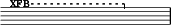
\includegraphics{../_assets/xfb-trimmed.png}
    &
    ``extremely fast bow'' spanner.
    \\[0.5cm]
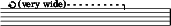
\includegraphics{../_assets/circle-trimmed.png}
    &
    circle bowing;
    one complete circle per notated duration.
    \\
\end{tabular}
%
\hfill
%
\begin{tabular}[t]{p{2cm} p{5cm}}
\textbf{XFB} & ``extremely fast bow'': very pronounced flautando;
    play with generous amounts of bow lightly skimming the string;
    retake bow irregularly as necessary;
    resulting color almost `fluorescent';
    only occurs at quiet dynamics.
    \\ 
\end{tabular}

\end{document}
